%!TEX root = ../../thesis.tex
\define{\chapterpath}{\allchapterspath/introduction}
\define{\imgpath}{\chapterpath/img}

\chapter{Introduction}
\label{chapter:introduction}
\minitoc

From robotic vacuum cleaners to self-driving car, smart home thermostat to autonomous trading, more and more autonomous intelligent systems are coming into our daily life, taking on their own decisions that can affect our everyday life. As such system becomes more and more advance and intricate, they also become more and more difficult to predict. As a direct consequence, it will be more and more difficult to explicitly get them to do what we want them to do. Their internal mechanisms can no longer be understood by a single person which makes the need to integrate simple, intuitive, and high-level interacting capabilities to those systems primordial.

We start by providing a small vision of what autonomous intelligent systems are nowadays and then present a brief overview of the main challenges involved when designing autonomous systems. We further explicit the need for such system to learn from their environment and present the major learning paradigms used nowadays. After focusing our analysis on learning paradigms based on interaction with human, we introduce the recent advances in interactive learning where the human and the learning system are in close interaction. Finally we identify and introduce the problem of interacting with a system without pre-coordination of communicative means. We call this challenge the problem of \textbf{fluid interactive learning} which is the main topic investigated in this thesis.

Most of our discussions will be articulated around the current trend of autonomous robots that are predicted to play an important role into our daily life in the coming century. However we would like the reader to keep in mind that an autonomous intelligent interactive system, such as a robot, can take many other form such as a virtual agent, a smartphone, or an intelligent prosthesis.

%%%%%%%%%%%%%%%%%%%%%%%%%%%%%%%%%%%%%%%%%%%%%%
%%%%%%%%%%%%%%%%%%%%%%%%%%%%%%%%%%%%%%%%%%%%%%
%%%%%%%%%%%%%%%%%%%%%%%%%%%%%%%%%%%%%%%%%%%%%%
%%%%%%%%%%%%%%%%%%%%%%%%%%%%%%%%%%%%%%%%%%%%%%
%%%%%%%%%%%%%%%%%%%%%%%%%%%%%%%%%%%%%%%%%%%%%%
\section{Autonomous intelligent systems around}

At home, workplaces or schools, an increasing amount of intelligent robotic systems are starting to be able to help us in our daily life (windows or vacuum cleaners, self-driving cars) \cite{gates2007robot} and in flexible manufacturing systems \cite{baxter} (Figure~\ref{fig:introduction:robots}). They are characterized by their ability to take important decisions autonomously, such as whether or not to engage at crowded road crossing. It is very different from the usual protective fences in industrial robots which creates several challenges related to safety, unpredictable environments, acceptability and usability by and adaptation to non-technically trained people. 

Most of the autonomous intelligent systems are developed with the aim to improve users quality of life and should therefore comply to the preferences of each users. My autonomous car should come take me at work at 6 p.m. and bring me back home. My vacuum cleaner should vacuum only the rooms I want at the time of the day I decided. My smart watch or smart glass should display the information that matters to me. My surveillance robot should patrol around my house following the specific pattern I envision.

\begin{figure}[!h]
    \centering
    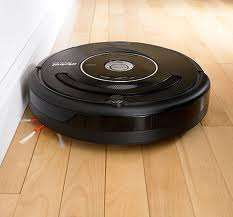
\includegraphics[height=0.2\columnwidth]{\imgpath/roomba.jpg}
    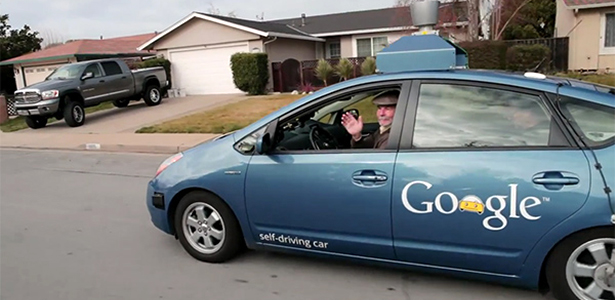
\includegraphics[height=0.2\columnwidth]{\imgpath/google_self_driving_car.jpg}
    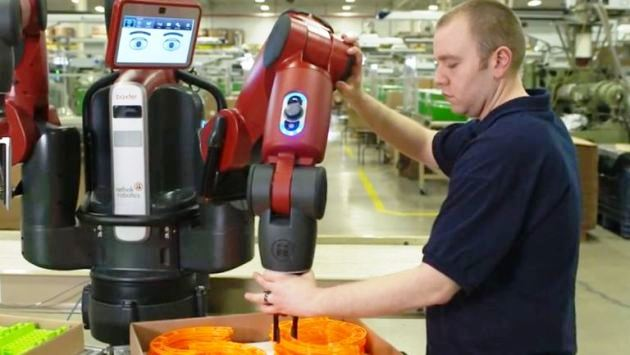
\includegraphics[height=0.2\columnwidth]{\imgpath/baxter_coworking.jpg}
    \caption{Three examples of nowadays autonomous intelligent robots. From left to right: a Roomba vacuum cleaner, an autonomous car from Google, and a collaborative robotic worker called Baxter.}
    \label{fig:introduction:robots}
\end{figure}

How can we balance autonomy and commitment in autonomous intelligent systems? In order to have machine performs complex task for us, that require complex sensing, acting and planning skills we need to endow them with the ability to make plans and learn from their day to day experience. Once such system as the ability to perform many different tasks in many different ways, the question of how to explicitly get these robots to do what we want becomes of crucial importance. The following section briefly introduce the many challenges associated to the design of autonomous intelligent machines.

%%%%%%%%%%%%%%%%%%%%%%%%%%%%%%%%%%%%%%%%%%%%%%
%%%%%%%%%%%%%%%%%%%%%%%%%%%%%%%%%%%%%%%%%%%%%%
%%%%%%%%%%%%%%%%%%%%%%%%%%%%%%%%%%%%%%%%%%%%%%
%%%%%%%%%%%%%%%%%%%%%%%%%%%%%%%%%%%%%%%%%%%%%%
%%%%%%%%%%%%%%%%%%%%%%%%%%%%%%%%%%%%%%%%%%%%%%
\section{Challenges}

As robots enter more and more into our daily life they will have to deal with our daily environment that is often unstructured and open-ended. In this section we identify and briefly present six main challenges of nowadays robotics: sensing, acting and planning, social interaction, morphology, adaptation and life long learning.

\subsection{Sensing and analyzing}

\question{How can a robot sense and make sense of its environment?}

Sensing start by developing advance sensors allowing the robot to collect information about the relevant features of its environment. Most of the work on sensor applied to robotic lies in vision and localization systems which are primordial for the robot to known where object are in the environment and where the robot it-self is in that environment. But having access to a raw image do not give the robot the ability to locate in a room. Some analysis of the raw sensors information is required to recognize objects in a scene \cite{filliat2007visual}, people in a room \cite{nakauchi2002social}, or the robot location \cite{durrant2006simultaneous, bailey2006simultaneous} and also to understand facial expression \cite{valstar2006fully}, gesture \cite{nickel2007visual} or gaze direction \cite{matsumoto2000algorithm}.

This problem is inherent to most of the modalities used in robotics nowadays. From sounds waves, robots may need to infer the location of speaker \cite{nakadai2002real,valin2003robust}, the recognition of a pronounced word \cite{rabiner1989tutorial}, and the emotional state of the speaker \cite{oudeyer2003production}. From touch, they should the texture \cite{howe1989sensing,nguyen2011texture}, hardness \cite{shikida2003active} or shape \cite{schneider2009object} of an object, avoid too strong impacts \cite{alami2006safe} , and even dose their physical contact with human \cite{nakagawa2011effect,miyashita2007haptic}. And from raw millimeter precision Lidar sensors, they should identify pedestrian, bicycle, car, truck position and their intention \cite{himmelsbach2008lidar}. In addition information from different sensors can be merge together to gain access to new kinds of information or gain precision in one specific estimate \cite{xiong2002multi}. 

\transition

However having access to high level and precise information from the environment is useless for a robot if it can not be used to act appropriately in the environment. In next section we present the challenge of acting and planning.

\subsection{Acting and planning}

\question{How can a robot affect its environment and plan its actions in our cluttered and dynamics environment?}

Acting starts by developing advance actuators allowing the robot to alter the current state of its environment. Most of our robot actuators today are motor based and produce many forms of motion from rotary movements. However being able to produce movements does not mean the robot will produce useful movements. As sensing requires analyzing, acting requires planning.

A robot that should evolve in our daily life should be able to move around our houses where many objects are constantly changing positions, with stairs, different floor's types and even human and animals moving around. Assuming the robot can sense and analyze every information needed to navigate, it still need to coordinate all its actuators in order to reach a goal. This coordination problem is especially difficult for problem like walking \cite{kajita20013d,lapeyre2011maturational} or grasping \cite{bicchi2000robotic} where many degrees of freedom are involved and should be synchronized in a proper way.

Acting is often an integral part of the sensing process, where sensors like cameras are mounted on articulated pan-tilt actuators to mimic human eyes. In this case the act of sensing is tightly coupled with the act of moving \cite{bajcsy1988active,lonini2013robust}.

\subsection{Interacting with social peers}

\question{How can a robot interact and communicate with humans?}

As robots are meant to help us in our daily life, they need to be able to interact with us, to understand us and be understood by us. To be understood a robot should act in a socially acceptable manner, adapt its behavior to the current context of interaction, express its current state by displaying familiar signs of emotion using on the appropriate modality.

Being social is also reacting correctly to the social signals sent by the other social beings. It requires the robot to sense and analyze touch, speech, gestures, gaze, facial expression, or other kinds of interfaces but also normative social rules such as appropriate distance of interaction \cite{strait2014let}, eye contact \cite{andrist2014conversational}, hand over \cite{moon2014meet}, or trajectory \cite{kruse2014evaluating} dynamics.

This multi-disciplinary study of social interaction between human and robot is the field of human-robot interaction (HRI) \cite{fong2003survey,dautenhahn2007socially,goodrich2007human}. An important challenge is to design and conduct human-robot interaction studies which allow to evaluate the objective and subjective usability and acceptability of the human-robot interaction \cite{scholtz2003theory,walters2005practical,young2011evaluating}.

\subsection{Design, morphology and appearance}

\question{What geometry, color, size, or shape should take a robot to be socially accepted among humans as well as efficient in its everyday activities?}

The morphology and appearance of a robot are properties that impacts all the previously defined challenges. The way the different parts of the body are design will affect the ease of the robot to perform a daily task. The way a sensor is located on its body will affect the sensing performance and its analysis. And the way a robot looks will affect its ability to tight up link with surrounding human could make the more technology advance robot worthless. We will highlight the influence of morphology and appearance for acting, sensing, and socially interacting using three using concrete example from the literature.

\paragraph{Better acting} The geometry and distribution of mass in the body has complex influences on biped locomotion. Several studies have for example explored the role of the foot and ankle morphology for biped walking on both human and robot, but the impact of various thigh shapes a robot dynamics \cite{lapeyre2013poppy}. This later work study the impact of a bio-inspired thigh, bended of 6 degree and with a geometry inspired by humans, on the balance and biped locomotion compared to a more traditional straight thigh. They have shown that the bio-inspired thigh allows the reduction of falling speed by almost 60\% and the decrease of the lateral motion needed for the mass transfer from one foot to the other by 30\%.

\paragraph{Better sensing} The design component of the body is also important for the sensing capabilities of the robot. As an example, the fingerprint while moving our finger on a textured surface enhance our ability to differentiate textures \cite{hollins2010somesthetic} compared to a smooth finger surface. By taking inspiration from the fingerprint properties, researcher have created an artificial finger that is more sensitive to textured surface \cite{candelier2011role}.

\paragraph{Better acceptability}

Effect of robot appearance on human-robot interaction is a widely investigated topic \cite{li2010cross, heerink2006studying}. One of its prominent characteristic is called the uncanny valley \cite{mori1970uncanny}, which state that the relation between human likeness of a robot and its perceived familiarity by human does not hold a linear relation. It states that familiarity increases with human likeness until a point is reached where a subtle deviations from human appearance and behavior create a unnerving effect, which is called the uncanny valley. More recent developments speculate that maybe even the most human-like androids, and even real human faces, are not liked as much as toy robots or humanoids. This effect has been called the uncanny cliff \cite{bartneck2007uncanny}.

\subsection{Adapt, adapt, adapt}

\question{How can a robot adapt to our open ended and dynamics environment \\ throughout its lifetime?}

Things change and a robot that is designed, built and programmed to live in todays words will have to learn new skills during his life time. It may even have to learn them right from the beginning, such as learning the language and habits of the community it leaves in. It may also break some of its parts, and will have to learn to deal with it or to adapt to the properties of the new replacement parts.

Therefore rather than trying to represent all human knowledge in our robots it seems more natural to endow them with the ability to learn. This idea has been formulated more than sixty years ago by Alan Turing \cite{turing1950computing} advocating that ``instead of trying to produce a programme to simulate the adult mind, why not rather try to produce one which simulates the child's?''. 
This precise line of research really began to be explored in the beginning of the century with the emerging field of developmental robotics \cite{weng2001autonomous,lungarella2003developmental} which ``aims at studying the developmental mechanisms, architectures and constraints that allow life long and open-ended learning of new skills and new knowledge in embodied machines'' \cite{oudeyer2012developmental}. 

While the idea of learning for machine is commonly accepted, developmental robotics is yet an emerging field inside the robotic and machine learning community. Most of the learning algorithm today do not take into account many aspects of the real life challenges robot should be able to face in our open-ended and dynamic environment. 

\paragraph{Open-ended environment} Most of the learning literature focus on abstract and well structure problems, where the researcher define in advance a representation well suited to the problem. But not every problem can be define in advance, as we learn to use smartphone which did not exist few years back, a robot should be able to learn how to use new systems without the need for an engineer to reprogram it, and this throughout their life time.

\paragraph{Lifelong learning} Lifelong learning can be define as the ongoing and self-motivated pursuit of knowledge and the ability needed to adapt to our everyday problems. Most of the learning literature do not consider learning as an ongoing activity. As an example, classification algorithms often need to have access to a batch of labeled examples which must therefore be collected by an engineer beforehand. But in order to adapt to our everyday problems embodied autonomous robots should be able to actively seek and select useful information in their environment. 

% maturational constraints biasing and constraining learning process

\transition

In the next section we describe the three main learning paradigms considered nowadays: learning from extrinsic motivation, intrinsic motivation, and social interaction.

%%%%%%%%%%%%%%%%%%%%%%%%%%%%%%%%%%%%%%%%%%%%%%
%%%%%%%%%%%%%%%%%%%%%%%%%%%%%%%%%%%%%%%%%%%%%%
%%%%%%%%%%%%%%%%%%%%%%%%%%%%%%%%%%%%%%%%%%%%%%
%%%%%%%%%%%%%%%%%%%%%%%%%%%%%%%%%%%%%%%%%%%%%%
%%%%%%%%%%%%%%%%%%%%%%%%%%%%%%%%%%%%%%%%%%%%%%
\section{Learning paradigms}

Hard coding control or planning solutions into robots is not a viable solution for robots that aims at entering into our daily life. Learning seems to be a more promising approach and many work have tackled this problem. Among them we can draw three main paradigms: \begin{inparaenum}[(a)] \item learning from extrinsic motivation, where an objective is given to the robot that should be either maximize or minimize, \item learning from intrinsic motivation, where the robot define its own objectives, and \item social learning, where a social agent which as already acquired some skills helps an other agent to acquired the same skills, it is characterized by a tight interaction loop between the two partners. \end{inparaenum} The following subsections provide a small introduction to the three paradigms.

\subsection{Learning from human defined objective function: extrinsic motivation}

Extrinsic motivations are driven by external rewards or punishments which arise from outside of the robot own control. It is a measure of fitness with respect to a given objective. For robots, these functions are usually defined by the engineer and the role of the learning system is to explore the environment and learn to minimize or maximize them. It can be a hard-coded pain like punishment useful for the robot to learn to avoid braking itself, a reward proportional to the position shift of the robot with respect to a predefined path to follow, or a boolean stating if a task is correctly executed or not. Famous examples include autonomous chess players \cite{newborn1997kasparov} and self-driving cars \cite{montemerlo2008junior}.

To maximize of minimize a fitness function, most of the algorithm rely on gradient based methods which allow to follow the slope of the fitness function until a local extrema is found. Some method ensure a convex fitness function which guarantee the extrema is global, other methods use a more global search, starting from different ``location'' on the fitness function to maximize their chances of finding the global extrema. Among others, we can refer to gradient descent (first order), newton's method (second order) \cite{battiti1992first}, but also to more global search algorithm such as particle swarm optimization \cite{kennedy1995particle,poli2007particle} or genetic programming \cite{goldberg1989genetic,nolfi1994evolve}.

\subsection{Self-directed learning: intrinsic motivation}

Intrinsic motivations are driven by an interest in the activities for their own sake which arises from within the robot and depends on its own internal operations rather than on external pressures or rewards. As for extrinsic motivation the robot should explore the environment but this time its objectives are not defined in advance by the engineer and is dynamically changing depending on the past experiences and current state of the robot. Intrinsic motivations \cite{oudeyer2007what} allow the robot to gain autonomy with respect to the open-ended challenges it may face into the real words. 

Various computational architectures have been proposed in the literature for implementing forms of intrinsic motivation \cite{schmidhuber1991adaptive,thrun1995exploration,huang2002novelty,kaplan2003motivational,marshall2004emergent,csimcsek2006intrinsic,sporns2006evolving,capdepuy2007maximization,schembri2007evolving,merrick2009motivated,baranes2009r}. There can be many different drive for a robot to explore and learn from its environment, such a reducing entropy or uncertainty, or maximizing learning progress. This latter form, driven by knowledge or skill acquisition, state that the agent should focus on what is not too hard to learn nor already known. It should focus on area where the learning progress is maximal. In others words, things starts getting boring for the robot as soon as they are predictable or impossible to predict (such as random noise), i.e. when there is no learning progress anymore, that is the first derivative of predictability is zero. This principle allowed to make interesting replication of observed phenomenon in living organism, such as on the the organization of early vocal development in infants \cite{moulin2013self}.

\subsection{Learning from others: social interaction}
\label{sec:intro:paradigms:social}

For a robots to be able to help in our daily activities, it should learn to perform various different task. As seen in previous subsections, one possible approach to this problem is to define an fitness function corresponding to each task and let the robot finding out how to optimize its performance. This process as two main flaws for real word application: \begin{inparaenum}[(a)] \item for most daily problems it is impossible for a non-expert user to write down a fitness function in the language of the machine, and \item even if a fitness function could be defined the almost infinite space of search in our environment makes it long and tedious to find an acceptable solution to most of the problems. \end{inparaenum} 

A good opportunity is to rely on the knowledge human already have on most situation of our daily life. On this basis, researcher investigate how a skill can be transfered from a human to a robot, this field of research is called social learning \cite{nehaniv2007imitation}. This field aims to create robotic systems teachable by non-technical users, i.e. \textbf{programmable for new tasks in novel environments} through \textbf{intuitive, flexible and personalized interactions}. Social learning allow to guide the robot towards correct learning situation, by, for example, providing good demonstrations of the task or assessing the robot actions.

This thesis focus more on the social learning paradigm, where two partners should interact together in order to fulfill a common goal. We will enter into more detail about social learning in section~\ref{sec:intro:social}, where we will identify three main social learning paradigms: \begin{inparaenum}[(a)] \item learning from human demonstration, where the robot learns by imitating the human actions, \item learning from human reinforcement, where the robot learn from assessments on its own actions provided by the user, and \item learning from instructions, where the robot learn from concrete instruction about what do to next provided by the user. \end{inparaenum}

\transition

The categorization of learning paradigms above in three categories does not reflect the many subfamilies that exist between these categories, including those that are shared among categories. It is meant to situate the learning paradigms into a more global picture, providing some interesting pointers for the interested readers. 

This thesis focus on the social learning aspects, where robots should learn by observing or being instructed by a human. Before entering into more details about the social learning paradigms in section~\ref{sec:intro:social}, we present three main problems identified in the machine learning literature.

%%%%%%%%%%%%%%%%%%%%%%%%%%%%%%%%%%%%%%%%%%%%%%
%%%%%%%%%%%%%%%%%%%%%%%%%%%%%%%%%%%%%%%%%%%%%%
%%%%%%%%%%%%%%%%%%%%%%%%%%%%%%%%%%%%%%%%%%%%%%
%%%%%%%%%%%%%%%%%%%%%%%%%%%%%%%%%%%%%%%%%%%%%%
%%%%%%%%%%%%%%%%%%%%%%%%%%%%%%%%%%%%%%%%%%%%%%
\section{Problem categories}

The three main paradigms define in previous section can be applied in many different kinds of problem. In machine learning, we can define three main categories of problem: \begin{inparaenum}[(a)] \item supervised learning, where the true nature of some data is known and is used to infer the nature of new ones, \item unsupervised learning, where some properties about raw data should be found, and \item reinforcement learning, where the system should maximize its cumulative reward. \end{inparaenum}

\subsection{Supervised learning}
\label{chapter:introduction:supervised}

Supervised learning is the problem of inferring a model from labeled training data. The inferred model can later be used for mapping new examples. It requires the learning algorithm to generalize from the training data to unseen situations. Most of the supervised learning problem are of two type: \begin{inparaenum}[(a)] \item classification problem, where the algorithm should differentiate example in categories, and \item regression problems, where the algorithm should estimate the relationship among variables.\end{inparaenum}

\paragraph{Classification}

Classification is the problem of identifying to which of a set of categories, called class, a new observation belongs. The training data are composed of a pair of input object, usually a a feature vector, and its associated class. As a example, the well known MNIST database of handwritten digits \cite{lecun1998mnist} is composed of raw images of handwritten digits paired with their associated symbolic digit. From a database composed of many such examples, the supervised learning algorithm should return a function able to predict the class, e.g. the digit, corresponding to a new raw digit image. Among others, classification algorithms include logistic regression, support vectors machines, or neural networks \cite{bishop2006pattern}. Some application domains are handwritten recognition for automatic mail direction \cite{plamondon2000online}, detecting cars and bicycle from Lidar sensors \cite{himmelsbach2008lidar}, or classifying aggregate of cells as cancerous or not \cite{furey2000support}.

\paragraph{Regression} 

Regression is the problem of estimating relationships among variables. Regression analysis is used to predict the value of some variables conditionally to the values of other variables, and to explore the forms of these relationships. Most of the regression algorithms, such as linear regression \cite{bishop2006pattern}, are parametric. It means that the fitted model is defined in terms of a finite, pre-defined number of parameters whose value should be estimated from the observation. Fitting a fixed function from a dataset is not always convenient as one would like to known the uncertainty of the predicted value. Therefore a common practice is to describe the regression function as a probability distribution, such as when using Gaussian process for regression \cite{rasmussen2006gaussian}. An application domain is inverse kinematics learning \cite{d2001learning}, where a robot should for example learn the mapping between its motor configuration and the spacial position of the tip of its arm.

\paragraph{} The purpose of fitting a model on data is to be able to prediction. The fitted model should therefore generalize to previously unseen situation. An algorithm that match too closely with the observed data is likely to describe random measurement error and may not generalize well. This problem is called over-fitting and usually appears when the model to fit is too complex or when the number of observation is small with respect to the number of parameters in the model. The opposite of over-fitting is called under-fitting and correspond to a model that generalize too much, usually using a simplistic model with too few parameters, such as using a linear function to model a quadratic function.

To evaluate the quality of a supervised learning algorithm with respect to over- and under-fitting, e.g. how accurately a classifier will perform in practice, it should be tested on previously unseen data that were not part of the training examples. A well known method is called cross-validation \cite{kohavi1995study}. It involves partitioning an initial dataset into several different subsets and using some of the subset(s) to train the classifier (called the training set) and testing the classifier on the remaining subset(s) (called the test set). To reduce variability, the process can be repeated with other subsets or combination of subsets. A classic approach is called ten-fold cross-validation and consist of splitting the original dataset in ten subsets, use nine in the training set, and the remaining one into the test set. As there is ten subsets, the process is repeated ten times and results averaged over the rounds.

\subsection{Unsupervised learning}

Unsupervised learning is the problem of finding hidden structure in unlabeled data. Even if there is no explicit error or reward to evaluate a potential solution, there is still predefined metrics which define what the terms \emph{structure} means. Finding an hidden structure is more looking from known patterns in unlabeled data.

It mostly applies in clustering task where a dataset is divided into subgroups of data which share common characteristic, such as a close proximity in the feature space. Among others, clustering algorithm include k-means and its generalized form the expectation maximization for Gaussian mixture \cite{dempster1977maximum}. Clustering method are widely used in recommender systems, especially in nowadays social networking service to identify group of users from a huge pool of user profile \cite{sarwar2002recommender}.

It also applies in feature extraction and dimensionality reduction problems where the algorithm should find a better, usually more compact, representation of the data without losing some of their properties. Among others algorithm, we can refer to principal component analysis (PCA) which linearly project a dataset into a subspace where dimension are minimally correlated \cite{jolliffe2005principal}. The new dimensions are called principal components. Linear projections are not always well suited for reducing dimensionality of some datasets which may lie on a non-linear manifold. Among others, non-linear dimensionality reduction algorithms include self-organizing map (SOM) \cite{kohonen2001self} which can be considered as the non-linear generalization of PCA.

\subsection{Reinforcement learning}

Reinforcement learning is the process of learning from rewards. The goal of the robot is to take action in its environment in order to maximize the cumulative reward received during its lifetime. The environment is usually modeled as a Markov decision process (MDP) \cite{sutton1998reinforcement}. When the MDP dynamics (also called transition probabilities) and the reward function (also called transition costs or gains) is known, dynamic programming proposes a solution to the problem of finding the optimal sequence of action to maximize cumulative rewards, this sequence of action is called the optimal policy. Dynamic programming equations are Bellman equations \cite{bellman1956dynamic} and Value Iteration (VI) algorithm \cite{sutton1998reinforcement} is a dynamic programming solution to a fully define, known in advance, RL problem.

But if the transition probabilities and the transition gains are unknown, like it is often in practical applications, the robot as to learn them by interacting with the environment, while trying to maximize cumulative rewards. Note that although the reward and transition probabilities are unknown they do exist and have to be learn by trying out. In that sense reinforcement learning differs from dynamic programming, as the solution will be found online, without planning before. But reinforcement learning uses learning concepts that are built on the dynamic programming, such as the SARSA (State-Action-Reward-State-Action) or the Q-learning algorithm \cite{rummery1994line,sutton1998reinforcement} that uses an update rule taking into account the observed reward instead of the true hidden one.

\paragraph{On-policy vs. Off-policy} In the world of reinforcement learning there are two categories of learning, the on-policy and off-policy learning. On-policy methods, such as SARSA \cite{rummery1994line}, estimate the value function of the policy generating the data. For example, the value function of acting randomly in the environment, or of performing always the same action. Off-policy methods, such as Q-learning, estimate the value function with respect to a policy different than the one the agent is using. As an example, Q-learning \cite{sutton1998reinforcement} estimates the value function relative the greedy policy.

\paragraph{Exploration vs. Exploitation} 
The goal of the agent is to maximize a cumulative reward and it might believe that a particular action in a particular state has a fairly high payoff probability. Should it choose that action all the time, or should it choose try to explore other states that may reward more? And the more time spent in exploring, the less time spent in collecting rewards, this is called the exploration vs. exploitation trade-off. 

Solutions to this problem depend on how long the agent is expected to play the game; the longer the game lasts, the worse the consequences of prematurely converging to a sub-optimal solution, and the more the robot should explore. It is call the exploration vs. exploitation trade-off and has been thoroughly studied through the multi-armed bandit problem \cite{berry1985bandit,audibert2009exploration}. Simple but successful methods for tackling the exploration vs. exploitation trade-off in reinforcement learning include the epsilon-greedy, softmax \cite{sutton1998reinforcement}, and R-max \cite{brafman2003r} methods. Curiosity based exploration \cite{schmidhuber1991curious,storck1995reinforcement,barto2004intrinsically,singh2005intrinsically} was also considered as well as method to learn or adapt the exploration strategies online \cite{mahmood2012tuning,Hester13aamas}.

\transition

The categorization of learning problems above in three categories does not reflect the many subfamilies that exist between these categories, including those that are shared among categories. It is meant to situate the learning problems into a more global picture, providing some interesting pointers for the interested readers. 

In next section we provide more details of the literature from the social learning paradigm presented in section~\ref{sec:intro:paradigms:social}, which we organized in three main groups: learning from human demonstrations, learning from human reinforcement, and learning from human instructions.

%%%%%%%%%%%%%%%%%%%%%%%%%%%%%%%%%%%%%%%%%%%%%%
%%%%%%%%%%%%%%%%%%%%%%%%%%%%%%%%%%%%%%%%%%%%%%
%%%%%%%%%%%%%%%%%%%%%%%%%%%%%%%%%%%%%%%%%%%%%%
%%%%%%%%%%%%%%%%%%%%%%%%%%%%%%%%%%%%%%%%%%%%%%
%%%%%%%%%%%%%%%%%%%%%%%%%%%%%%%%%%%%%%%%%%%%%%
\section{Robot learning from social interaction with humans}
\label{sec:intro:social}

As stated before, it is often easier to acquire a new skill if someone that already acquired that skill teach us how to do it. In robotics, we investigate how knowledge can be transmitted from humans to robots through social interaction. This way human users can interact with machines without knowing how to program or how to define a fitness function for a particular task. They rather use speech, gesture and provide demonstration of the skills which has the advantage of being an intuitive way for humans to instruct robots. 

In the following of this section we present three main social learning paradigms: \begin{inparaenum}[(a)] \item learning from human demonstration, where the robot learns by imitating the human actions, \item learning from human reinforcement, where the robot learn from assessments on its own actions provided by the user, and \item learning from human instructions, where the robot learn from concrete instruction about what do to next provided by the user. \end{inparaenum}

\subsection{Learning from human demonstrations}

Learning from human demonstrations, also called programming by demonstration or learning by imitation, is the process of learning from practical examples of how to perform a specific skill \cite{schaal1999imitation,argall09survey,lopes10imitationchapter}. Demonstrating a task to a robot is more intuitive for the user than directly programming a behavior by writing lines of code. But creating a robot that learn from example requires to solves many problem with respect to the algorithm capable of inferring the task from the provided demonstrations but also to the way the robot can select and understand what part of the environment and of the interaction are relevant to the demonstrated task.

Four central questions were defined as who, when, what, and how to imitate \cite{nehaniv2000hummingbirds}:
\begin{itemize}

\item \textbf{Who} to imitate refers for example to the problem of finding which person in a group in more suited to provide correct demonstration or to identify that a person is currently providing demonstration. This question has not been throughly investigated in the literature so far. One of the few work tackling this problem consider a finite set of teacher and select the most appropriate one using intrinsic motivation processes based on the learning progress metric \cite{Nguyen2012PJBR}, which allow the robot learner to take advantage of the different levels of skills each teacher provide.

\item \textbf{When} to imitate refers for example to problems of social coordination between two partners, such as the turn-taking ability. For example, this aspect has been investigated in human-robot drumming activities where turn-taking and role switching are important component of a successful interaction \cite{weinberg2006robot,kose2008emergent}. The when question also applies for cases where the robot should decide whether to try to imitate its human partner or to explore the environment by itself. The work presented in previous paragraph \cite{Nguyen2012PJBR} makes also use of curiosity to select whether to self-explore, mimic or emulate using a curiosity based selection method.

\item \textbf{What} to imitate refers to the dilemma between imitation at the action level or emulation at the effect level. It is the problem of identifying the important aspect of the demonstrations. At the action level, the aim of the robot would be to reproduce the demonstrator action in the same way and in the same order. At the effect level, the robot should understand the underlying purpose associated to the action of the human. Such as when fixing a shelf on a wall using nails, the important aspect could be to have the shelf fixed but nails could be replaced by screw, or when poring water into a glass, to specific position of the arm may or may not be an important aspect of the demonstration, e.g. in hostelry it would matter while at home it may not be relevant. 

The latter problem of identifying the effect level of imitation depends on the context in which the interaction takes place. In particular the concept of affordances \cite{gibson1986ecological} --- which encode the relation between actions, objects and, effects --- is of primordial importance for the robot to be able to reproduce demonstration at the effect level. Several works have consider affordances for human-robot learning, among others they have been used to recognize demonstrations, decompose them in a sequence of subgoals and finally reproduce them \cite{macl07affimit}. Affordances have also been learn, in \cite{montesano2008learning}, Montesano et al. present a robot that, by interacting with several objects, is able to extract relation betweens its actions, the objects, and the effects it produces using Bayesian inference methods. 

Other sources of information have been used to infer which parts of a demonstration are more relevant, such as the temporal differences of demonstration parts. Pauses during interaction have been shown to be linked to important key points in a task demonstration, and allow to extract subgoals or determine when a task is completed \cite{theofilis2013temporal}.

\item \textbf{How} to imitate refers to the problem of determining how the robot will actually perform the behavior so as to conform with the metric identified when answering the what to imitate question. When the demonstration is only relevant at the effect level, the robot can solve the task by its own mean as soon as the end result, e.g. the end configuration of objects, is correct. However when the imitation is important at the action level, differences between robot and human morphology and capabilities makes solving the how question not straightforward.

This latter issue is referred as the correspondence problem \cite{nehaniv2002correspondence}, which the problem of mapping between the demonstrator and the imitator. This problem is obvious between a human and a robot which do not share the same body characteristic, but it also apply between two human being that do not share the exact same morphology (size, strength) but also the same sensing abilities as our individual sensory experience are certainly not experienced the same way.

% we experience this problem often in our daily life. For example when we need to inform someone else that some eyelid fall on his/her cheek, we often mimic the action of removing the eyelid. But, due to the mirror effect, if I mimic removing the eyelid on my left cheek, does it means the person has one on its left or right cheek. Not surprisingly this problem applies to human-robot interaction too.

At the motor level, some work have addressed this question by for example having a robot imitating the body posture of a human demonstrator. To do so the robot can not reproduce the angle between each articulation as the resulting posture is likely to be different but more importantly the robot is likely to lose its balance and fall. The problem is therefore for the robot to copy the human posture as closely as possible while maintaining its balance \cite{hyon2007full,yamane2009simultaneous}. 

At the sensory level, a typical example is for two agent to agree on the name of specific colors. Considering two robots with different cameras, how can they communicate and agree on they respective perception. Several theoretical work have addressed this issue \cite{cangelosi2001adaptive,steels2005coordinating} that are closely related to language acquisition problems which we will discuss in chapter \ref{sec:related:language}.

\end{itemize}

Those four questions remains widely open challenges and are solved in practice by constraining the interaction between the human and the robot and by defining in advance what is relevant in the demonstration. In many cases the demonstration are collected beforehand and sent to the learning algorithm in a batch way.

Among others, algorithms for learning by demonstration include regression methods based on mixture models that allow to generalize trajectories from examples \cite{calinon07}. Inverse reinforcement learning \cite{Abbeel04icml} is an other popular method that is looking for the hidden reward function the demonstrator is trying to optimize based on the provided demonstration.

One of the most impressive achievement of the past decade used inverse reinforcement learning methods for the learning of aerobatic helicopter flight. Demonstration were provided by an expert pilot teleoperating, i.e. flying, the helicopter to help finding its dynamics and the fitness function corresponding to different maneuvers such as flip, roll, tail-in and nose-in funnel \cite{abbeel2007application}.

\subsection{Learning from human reinforcement}

An other way to help a robot improves its performance on a specific skill is to provide some feedback on its actions. This social learning paradigm has share many aspects with reinforcement learning problems, however the interactive component create more ambiguous situation. 

As for learning from demonstration, the robot should be able to infer to which part of its past actions the human feedback relates to, but may also need to differentiate between different levels of feedback as some actions may be mandatory to complete the task while others may just be preferences from the users. In addition the user could make mistakes in its assessment or may not perceive the problem as it is modeled by the robot, therefore making inconsistent feedback. As an example, it has been shown that feedback signals from human is frequently ambiguous and deviates from the strict mathematical interpretation of a reward used in reinforcement learning \cite{thomaz2008teachable,Cakmak2010optimality}.

Therefore, while reinforcement learning algorithm as been initial used for robot learning from human generated rewards \cite{thomaz2008teachable}, more recent works started to investigate how to additionally learn the way the human are providing feedback \cite{knox2009interactively}. I would actually argue that learning from human reinforcement is more related to inverse reinforcement learning than to reinforcement learning. Indeed, the goal of the robot should better be to find the hidden reward function that explains the assessment of the human teacher than to maximize the rewards, or positive assessments, given by the user. We will enters those issues into more details in the next chapter.

As for learning from demonstration, most of the current works consider predefined and restricted interaction so as to be able to map easily the human reinforcement with the robot's actions.

\subsection{Learning from human instructions}

Providing feedback to the robot becomes restrictive as the space of possibles grows. If the robot has to try out all possible actions before finding the ones that elicit a positive feedback, the interaction is doomed to fail; especially for sequential problems such as chess or video games. For such cases it would be better if the human teacher could provide instruction directly to the robot \cite{breazeal2004tutelage}.

Due to the high-level nature of concrete instruction, learning from instruction is often applied with robots that are already equipped with planning skills. But were a fitness function is hard to define, or when the search space is too big to be explored efficiently. For example, in \cite{lockerd2004tutelage}, the robot Leo already knowns how to press a button before the interaction starts. The robot learns the task of swithing buttons on from human instructions, and when a new button is introduced the robot autonomously generalizes from the instruction and presses all buttons, instead of pressing only the one it was instructed to in the first place. 

As for other method, the robot should be able to infer to which part of the environement matters for the instructions, if the instructions can be generalized or not to other objects in the environement, if the instructions are related to what the robot should do next or what it should have done before, in which referential are direction instruction given, or even if the user is really paying attention to the scene. And as for other methods, most of the current works consider predefined and restricted interaction so as to be able to map easily the human instruction with the current important aspect of the environment and of the interaction.

As for learning from demonstration or learning from human reinforcement, learning from instructions could also be considered as an inverse reinforcement learning problem. One way is to consider instructions as demonstration and use learning from demonstration technics , another way is to formulate the problem such that the robot's goal is to find the hidden reward function that explains the instruction of the human teacher.

% \transition shared attention far from reach but people in interactive learning are trying to integrate the human component in the loop In the line of Tomasello's research, we argue that joint attention is much more than simultaneous looking because it implies a shared intentional relation to the world. This requires skills for attention detection, attention manipulation, social coordination and, most importantly, intentional understanding. In line with Tomasello's views (Tomasello, 1995, Tomasello et al., 2004), we argue that joint attention must be discussed in the context of interactions between intentionally-driven agents. In that sense, joint attention is much more than gaze following or simultaneous looking. By formalizing attention as intentionally-directed perception and joint attention as a coupling between two intentional actions, we identify four complementary prerequisites that underly the capacity for joint attention. \cite{kaplan2006challenges} skills to understand, manipulate and coordinate attentional behavior 

\transition

The categorization of learning paradigms above in three categories does not reflect the many subfamilies that exist between these categories, including those that are shared among categories. It is meant to situate the social learning problem in a more global picture, providing some interesting pointers for the interested readers. 

As we noticed, in most of the above presented work, the human and the robot had no direct interaction with the robot, or few well controlled interactions. For example, the human demonstrations are provided in a batch perspective where data acquisition is done
before the learning phase. The properties of teaching interactions with a human in the loop was not yet considered in depth, and this issues have began to be addressed in a subfield called \emph{interactive learning}  which combine ideas of social learning with extrinsic and intrinsic motivated learning. Where the robot acquires a form of autonomy with respect to how to deal with the human in the loop. This separation between this section and interactive learning is a bit arbitrary, we mainly want to highlight the fundamental difference between system that learn from pre-recordeed, open-loop, and  well controlled interactions from those which tries to close the interaction loop and allow more flexibility in the interaction process..

%%%%%%%%%%%%%%%%%%%%%%%%%%%%%%%%%%%%%%%%%%%%%%
%%%%%%%%%%%%%%%%%%%%%%%%%%%%%%%%%%%%%%%%%%%%%%
%%%%%%%%%%%%%%%%%%%%%%%%%%%%%%%%%%%%%%%%%%%%%%
%%%%%%%%%%%%%%%%%%%%%%%%%%%%%%%%%%%%%%%%%%%%%%
%%%%%%%%%%%%%%%%%%%%%%%%%%%%%%%%%%%%%%%%%%%%%%
\section{Interactive Learning}


However non-expert users might have very
different preferences and predefined instructions might not be
well accepted. lies at the interaction of those domains + autonomy

bootstrapping further intrinsically motivated learning \cite{nguyen2011bootstrapping}
not a passive absorber of knowledge


A typical example, that I heard from Thomas Cederborg, is the case of a cleaning robot that could

demonstration, human generated reward

Underlying all IRL works is the assumption of a consistent reward function. When demonstrations are provided by multiple experts, this assumes that all experts optimize the same objectives. This is constraining and does not exploit the variability of ways in which humans may solve the same task. Recent IRL works consider multiple experts and identify multiple different reward functions (Choi and Kim 2012; Tanwani and Billard 2013). This allows the robots to learn multiple (albeit suboptimal) ways to perform the same task. The hope is that this multiplicity of policies will make the controller more robust, offering alternative ways to complete the task, when the context no longer allows the robot to perform the task in the optimal way. 

. LfD-PbD techniques assume that all the demonstrations are good demonstrations and researchers generally discard data that are poor proxy of what would be deemed as a good behavior. Recent work has begun to investigate the possibility that demonstrations corresponding to failed attempts at performing the task may be useful for learning (Grollman and Billard, 2011; Ray et al. 2013).

Perceptual learning and task learning can both benefit from user interaction in many different ways. On the one hand, if the interaction protocol and context, is well defined it is possible to acquired grounded perceptual data. On the other hand, if the human and the machine understand each others, the human can explain or guide the machine, which may reduce learning time or even enable the machine to learn task difficult to write down as an objective or reward function.

This leaded to interesting results concerning the behavior of human in such situation.

People will not always respect predefined conventions. Several studies discuss the different behaviors naive teachers use when instructing robots \cite{thomaz2008teachable,Cakmak2010optimality}. An important aspect is that the feedback is frequently ambiguous and deviates from the mathematical interpretation of a reward or a sample from a policy. For instance, in the work of \cite{thomaz2008teachable} the teachers frequently gave a positive reward for exploratory actions even if the signal was used by the learner as a standard reward. Also, even if we can define an optimal teaching sequence, humans do not necessarily behave according to those strategies \cite{Cakmak2010optimality}. For more studies on how humans teach robots see \cite{thomaz2009learning,kaochar2011towards,knox2012humans}. These studies show that even when using well defined protocols, it is important to consider how different instructions can be used for learning. 

Nevertheless the real problem is somewhat even more complicated. Figure shows this complexity. When observing the robot behavior the user will provide some instructions, using vocal commands for instance. If their meanings are known and the speech recognition system works then they can be directly translated into learning data for the task learning algorithms. But in general, it is important to consider that there can be errors in the recognition system, even systematic when taking into account accents, and that people might be more comfortable to use different, not predefined, words. The problem now becomes that the meaning of these new instructions can not be easily recovered if the task that is being learned is not known.

However most of those systems have not considered in depth the properties of teaching interactions with a human in the loop. The demonstrations are provided in a batch perspective where data acquisition is done before the learning phase. Those issues have began to be addressed in works studying \textit{interactive learning} \cite{kaplan2002robotic,nicolescu2003natural,Breazeal2004,thomaz2008teachable}, which combines the ideas of learning from demonstration, learning by exploration and tutor feedback. Under this approach, the teacher interacts with the robot and provides extra feedback or guidance. In addition, the robot can act to improve its learning efficiency. Recent developments have considered: extra reinforcement signals \cite{thomaz2008teachable}, action requests \cite{macl09airl}, disambiguation among actions \cite{chernova09jair}, preferences among states \cite{Mason2011}, iterations between practice and user feedback sessions \cite{judah2010reinforcement} and choosing actions that maximize the user feedback \cite{knox2009interactively}.

Interactive learning \cite{nicolescu2003natural,breazeal2004tutelage} aims at developing systems that can learn by practical interaction with the user and finds applications in a wide range of fields such as human-robot interaction, tutoring systems or human-machine interfaces.
This type of learning combines ideas of learning from demonstration \cite{argall09survey}, learning by exploration \cite{thrun1992efficient} and tutor feedback \cite{kaplan2002robotic}. Under this approach the human teacher interacts with the machine and provides extra feedback or guidance. 

In addition, the device can act to improve its learning efficiency.
Approaches have considered: extra reinforcement signals \cite{thomaz2008teachable}, action requests \cite{lopes2009active}, disambiguation among actions \cite{chernova09jair}, preferences among states \cite{Mason2011}, iterations between practice and user feedback sessions \cite{judah2010reinforcement}, and choosing actions that maximize the user feedback \cite{knox2009interactively}. 

\subsection{Online interactive learning}

\cite{akgun12hri}

learning by reading instruction books


\subsection{How people teach robots}

\subsection{User modeling and ambiguous protocols}

\cite{macl11simul}

\subsection{Ambiguous signals}

\subsection{Active learner}

\subsection{Active teacher}


find some framework and cite thomas \cite{cederborg2013language}

Perceptual learning and task learning can both benefit from user interaction in many different ways. On the one hand, if the interaction protocol and context, is well defined it is possible to acquired grounded perceptual data. On the other hand, if the human and the machine understand each others, the human can explain or guide the machine, which may reduce learning time or even enable the machine to learn task difficult to write down as an objective or reward function.




This thesis lies around those challenges. We identified one important assumtion made in all those experiments. The facts that the human and the robot are assuemd to be able to undertasn each others on one level or an other before the interaction can begin. Whether the meaning of the social signals are known and the robot should infer the task, or the task is known and the robot should infer some characteristic of its human partners, wheter the mapping between some communicative signals and their meaning, or the frequeccy to which it tends to use some words.


A usual assumption in such
systems is that the learner and the teacher share a mutual
understanding of the meaning of each others' signals, and in
particular the robot is usually assumed to know how to interpret
teaching instructions from the human. In practice, the range
of accepted instructions is limited to the one predifined by the
system developer.

 We believe that robots should themselves be
able to adapt progressively to every user's particular teaching
behaviors at the same time as they learn new skills

%%%%%%%%%%%%%%%%%%%%%%%%%%%%%%%%%%%%%%%%%%%%%%
%%%%%%%%%%%%%%%%%%%%%%%%%%%%%%%%%%%%%%%%%%%%%%
%%%%%%%%%%%%%%%%%%%%%%%%%%%%%%%%%%%%%%%%%%%%%%
%%%%%%%%%%%%%%%%%%%%%%%%%%%%%%%%%%%%%%%%%%%%%%
%%%%%%%%%%%%%%%%%%%%%%%%%%%%%%%%%%%%%%%%%%%%%%
\section{The challenge of fluid interactive learning}


in all the previous work demonstrated the interactino in done ont he basis that people know what the other person is saying, doing, stuffing. The interaction, while behing sometime interactive as strong known component respective to the meaning to communicative signals. we aim at removing that.


How can a robot learn to interpret our different modes of communication? 

Interactive learning combines the ideas of learning from demonstration, learning by exploration and tutor feedback. Two widely explored subfields are:
\begin{itemize}
\item \textbf{Interactive perceptual learning} in which the system learns to discriminate between perceptual events via the help of a human partner. If the interaction protocol and context is well defined it is possible to acquired grounded perceptual data. It implies \textbf{the machine is aware of the communicative goal of the human}.
\item \textbf{Interactive task learning} in which the system learn to increase its performance with respect to an objective or a reward function via the help of a human partner. If the human and the machine understand each others, the human can explain or guide the system, which may reduce learning time or even enable the machine to learn task difficult to write down as an objective or reward function. Therefore a usual assumption is that \textbf{the machine understands the meanings of human' s  communicative signals}.
\end{itemize}

Their respective assumptions makes those two lines of research incompatible. On the one hand, working on perceptual learning, i.e. learning the signal-to-meaning mapping, requires the machine to know the task. On the other hand, teaching a new task to a machine requires to already know the signal-to-meaning mapping. Consequently it is impossible for a user to instruct --- from scratch --- a machine using his own preferred teaching signals, the user must comply to the use of predefined ones or go through a calibration procedure.

Unknown signals, unknown tasks

A usual assumption in such systems is that the learner and the teacher share a mutual understanding of the meaning of each others' signals, and in particular the learning agent is usually assumed to know how to interpret teaching instructions from the human. In practice, this problem can be solved due to two simplifications. On one hand, the range of accepted instructions is limited to those predefined by the system developer. This approach, commonly used in human-robot interaction, lacks flexibility and adaptation to user specificities and, consequently, may not be well accepted by non-experts users with different preferences. 
%
On the other hand, sometimes it is not enough to predefine the instruction sets and it is necessary to perform a calibration phase to map raw signals such as speech or brain activity to the meaning. This is usually done using an ad-hoc protocol to collect labeled samples of the user communicative signals. This process must be well controlled to ensure signals are associated to the true intended meaning of the user.

The previous engineering solution is needed due to the chicken egg nature of the problem. In order to teach a system a new skill, it needs to understand the human instructions. And, in order to understand this feedback, the system must have some interaction with the human (e.g. through a controlled task as done in the calibration process) to learn what the instructions mean. 

Few works have studied and developed interactive learning systems that can learn both the meaning of symbols and the task simultaneously. In human-robot interaction Griffiths et al. \cite{griffiths2012bottom} conducted an experiment with humans learning the meaning of unknown symbolic teaching signals. Lopes et al. \cite{macl11simul} presented sequential task experiments considering symbolic teaching signals and requiring a bootstrap with known signals. Grizou et al. \cite{grizou2013robot} extended their system for non-symbolic teaching signals while removing the need for bootstrapping with known signals. Non-invasive brain-computer interfaces (BCIs) have also looked at this problem, since they usually require user-dependent calibration and have to deal with the EEG brain signals non-stationarities. These facts, together with the poor signal-to-noise ratio of the EEG, make the EEG self-calibration one of the most challenging ones. Specifically, for P300 spellers, Kindermans et al. have shown that it is possible to exploit the repetition of signals together with prior information  \cite{Kindermans2012a,Kindermans2012b} to calibrate the system while using the speller.


While research on robot learning from human interaction has flourished in the last ten years, most work has focused on how to extract statistical \textit{task models} from human teachers following a fixed pre-defined teaching protocol (e.g. using a pre-defined button for ``good'' or ``bad'' feedback or using ad-hoc words for guidance with a trained speech recognition and dialog system). Thus, a usual assumption is that the learner and the teacher share a mutual understanding of the meaning of each others' instructions, and in particular the robot is usually assumed to know how to interpret instructions from the user. In practice, the range of accepted signals is limited to the one predefined by the system developer. Also, it is often assumed that instructions are noiseless and can be directly used as a feedback signal for a learning algorithm. The question of how a robot can learn to interpret personalized and potentially noisy teaching signals, i.e. learn \textit{instruction models}, has been much less explored.

We can now define a general scientific challenge: \textit{Can a robot learn a new task if the task is unknown and the user is providing unknown instructions? Which are the constraints and mechanisms that could provide this flexibility in interactive task learning?} There are two important dimensions in such questions: 1) which are the computational machine learning algorithms and formalisms that are needed for this goal? 2) how to integrate them within real-world meaningful human-robot interaction such that usability and acceptability can be evaluated in user studies. Given the complexity and novelty of these issues, this article focuses on the first dimension, elaborating a formalism as well as algorithms that have good properties to address the broader challenge. While we present an exepriment with a real robot and discuss the second dimension in the discussion section, more thorough real-world user studies will be achieved in future work. Yet, we believe the theoretical work presented in this article can constitute an important first step towards flexible personalized teaching interfaces, and thus towards what we may call \textbf{fluid interaction learning}, a key for the future of personal robotics.

In the following, we present a system able to learn the meaning of instruction signals provided by a user using unlabeled speech while learning a task using inverse reinforcement learning. Our contributions are:
\begin{itemize}
    \item a learning algorithm that learns how unknown sub-symbolic instructions signals can be translated in a meaningful teaching signal (among a repertoire of possible ones) that can be used for learning a task (within a space of possible tasks);
    \item a learning algorithm that simultaneously learns the meaning of the instructions and a new task;
    \item an extension of uncertainty based planning in the context of IRL;
    \item tests with robotic systems using voice commands provided by a user using different representations: a finite MDP and an MDP with continuous state representation.
\end{itemize}

After detailing the related work in Section, we provide in Sectiondetails on the algorithm for learning tasks from unknown instructions. Section describes a set of experiments, where we will evaluate the algorithm in different settings. Section introduces an uncertainty based planning algorithm for efficient learning and we show the corresponding results in Section. Finally, we will discuss the main limitations of this work and suggest some future lines of research in Section. 


Our approach is based on a discretization of the possible tasks into a finite number. Each task assigns different expected meanings to the instruction provided by the user. The machine solves the most likely task according to a pseudo-likelihood function computed using the corresponding task labels. The experimental results, both synthetic and based on real EEG data, show that in order to simultaneously recover the meanings and solve the task it is of paramount importance to take into account the uncertainty on both task and signal space.

In the following section, we present the set of assumptions and algorithmic details of our system. Then we introduce the specificity of the uncertainty inherent to our problem using an intuitive example and present the details of our action selection method. Finally we present a set of simulated experiment showing that 
\begin{inparaenum}[a)]
\item our action selection method is reliable and improved over other methods
\item our algorithm scale to the use of high dimensional signals coming from previously recorded brain signals
\item by being operational from the first step, as opposed to calibration procedure, we can estimate the correct task as soon as sufficient evidence has been collected.
\end{inparaenum}

This work is particularly relevant for system requiring an individual adaptation to the user. For instance brain-computer interfaces (BCIs) are systems capable of decoding neural activity in real time, thereby allowing a machine to be directly controlled by thought. Such interfaces must be highly customized to adapt to each user brain signals. It often requires a fastidious calibration procedure, where the user is asked to repeat hundreds of time the same thought process in order to collect labeled data used to train a decoder, also called classifier.

%%%%%%%%%%%%%%%%%%%%%%%%%%%%%%%%%%%%%%%%%%%%%%
%%%%%%%%%%%%%%%%%%%%%%%%%%%%%%%%%%%%%%%%%%%%%%
%%%%%%%%%%%%%%%%%%%%%%%%%%%%%%%%%%%%%%%%%%%%%%
%%%%%%%%%%%%%%%%%%%%%%%%%%%%%%%%%%%%%%%%%%%%%%
%%%%%%%%%%%%%%%%%%%%%%%%%%%%%%%%%%%%%%%%%%%%%%
\section{Thesis Statement}

In this dissertation, I will advance the following thesis:

\begin{quote}
Under specific conditions, it is possible to start interacting with a device without pre-coordinating on the signals used for communicating specific meanings neither on what the device should aim for.
\end{quote}

%%%%%%%%%%%%%%%%%%%%%%%%%%%%%%%%%%%%%%%%%%%%%%
%%%%%%%%%%%%%%%%%%%%%%%%%%%%%%%%%%%%%%%%%%%%%%
%%%%%%%%%%%%%%%%%%%%%%%%%%%%%%%%%%%%%%%%%%%%%%
%%%%%%%%%%%%%%%%%%%%%%%%%%%%%%%%%%%%%%%%%%%%%%
%%%%%%%%%%%%%%%%%%%%%%%%%%%%%%%%%%%%%%%%%%%%%%
\section{Thesis Outline}

The purpose of this manuscript is to explain the problem of learning from unlabeled interaction frames and to provide an intuition on how to solve this problem. I will introduce the most important aspects of the work by simple, hopefully intuitive, visualization of the problem and of the specific properties we exploit. My aim is therefore to endow the interested readers to implement their own version of the algorithm with the tools they are more familiar with.

In chapter~\ref{chapter:relatedwork}, I will present an overview of the related work which span from language acquisition to brain computer interfaces.

In chapter~\ref{chapter:humanexperiment}, I will introduce a new experimental setup to study the co-construction of interaction protocols in asymmetric collaborative tasks with humans. By presenting preliminary results based on this setup, I will derive interesting lessons for our problem. This work on human experiment is a joint collaboration with Anna-Lisa Vollmer and Katharina J. Rohlfing. 

In chapter~\ref{chapter:lfui}, I will introduce in more specific terms the problem and provide a visual intuition on what properties we will exploit. I will continue by formalizing the problem in a probabilistic framework, describe how particular brick of the problem are implemented and present results from a robotic pick and place scenario.

In chapter~\ref{chapter:planning}, I will introduce the problem of planning related to the problem and provide a visual intuition on what properties we should track. I will continue by defining the uncertainty measure used in the planning process and demonstrate on a 2D grid world problem the efficiency of the method with respect to other planning strategies.

In chapter~\ref{chapter:bci}, I will present an application of the algorithm to a BCI scenario where a subject control an agent on a grid. We will describe online experiment showing that our algorithm allow our subjects to start controlling the device without any calibration procedure and by mentally assessing the device's actions. This work on BCI is a joint collaboration with I{\~n}aki Iturrate and Luis Montesano.

In chapter~\ref{chapter:limitations}, I will discuss the limitation of the work and exemplify, using simulated experiments, direction which could be pursue to overcome them.

